\newpage
\hypertarget{subSec:setupParser}{}
\subsection{Setting up the Parser}
\genHeader

We need some content here so that we don't just dive right in\ldots explain how the parser works? (WITH ANTLR)

\begin{itemize}

% \item[$\blacktriangleright$] Expand each of cour generated folders, and take a look at each of the \texttt{Moflon} and \texttt{Moca} libraries which reference
% the jars required for each of the project's dependencies (Fig.~\ref{eclipse:generatedAdapter}).
% 
% \begin{figure}[htpb]
% \begin{center}
%   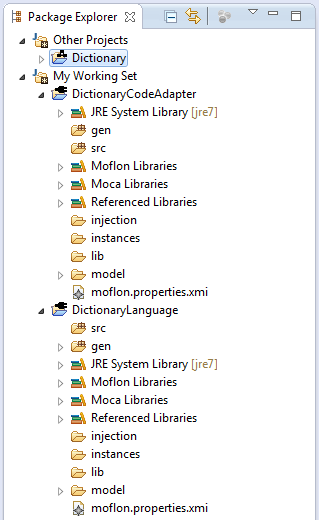
\includegraphics[width=0.4\textwidth]{eclipse_generatedAdapter}
%   \caption{figureCaption}
%   \label{eclipse:generatedAdapter}
% \end{center}
% \end{figure}

\item[$\blacktriangleright$] Right-click on \texttt{DictionaryCodeAdapter} and navigate to ``eMolfon/ Add Parser/Unparser'' (Fig~\ref{eclipse:contextParser}).

\begin{figure}[htpb]
\begin{center}
  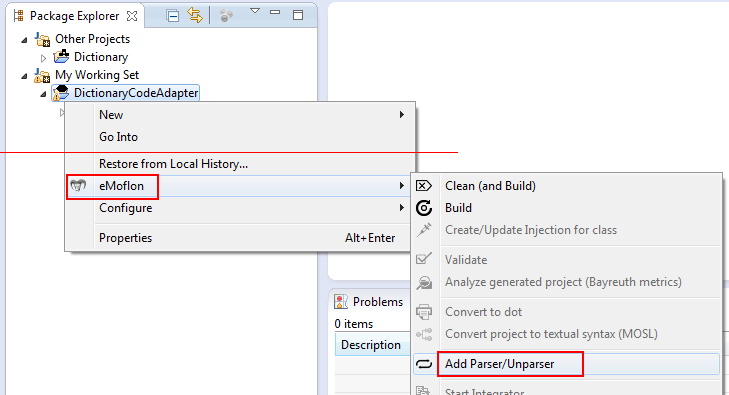
\includegraphics[width=0.9\textwidth]{eclipse_contextAddParserUnparser}
  \caption{figureCaption}
  \label{eclipse:contextParser}
\end{center}
\end{figure}

\item[$\blacktriangleright$] In the parser dialogue, enter ``dictionary'' as the \texttt{File extension}, and confirm \texttt{Create Parser} and \texttt{Create
Unparser} with \texttt{ANTLR} are selected as the corresponding technology in both cases (Fig~\ref{eclipse:wizardParser}). Affirm by pressing \texttt{Finish}.

\begin{figure}[htpb]
\begin{center}
  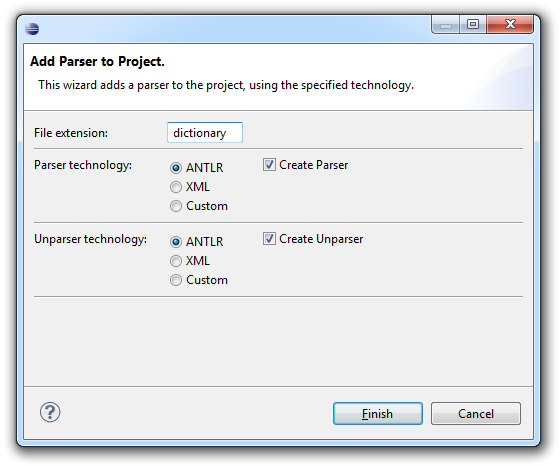
\includegraphics[width=0.8\textwidth]{eclipse_wizardParser}
  \caption{figureCaption}
  \label{eclipse:wizardParser}
\end{center}
\end{figure}

\item[$\blacktriangleright$] If everything has been installed and completed without error, parser and unparser stubs should be generated under
\texttt{DictionaryCodeAdapter}, where \texttt{ANTLR} automatically built the corresponding Java code as depicted in Fig.~\ref{eclipse:generatedParser}.

\item[$\blacktriangleright$] Your workspace is now fully prepared, and ready to start transforming from a textual file source into a \texttt{Dictionary} model!

\begin{figure}[htpb]
\begin{center}
  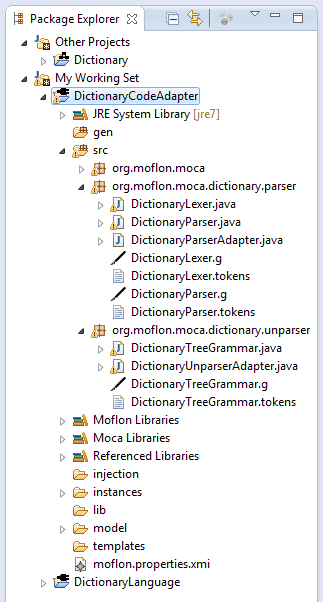
\includegraphics[width=0.4\textwidth]{eclipse_generatedParser}
  \caption{figureCaption}
  \label{eclipse:generatedParser}
\end{center}
\end{figure}

\item[$\blacktriangleright$]  {\bf self: update TGGMain and MocaMain (generated eMoflon files) so that tgg runs a round trip}

\end{itemize}
